%%%%%%%%%%%%%%%%%%%%%%%%%%%%%%%%%%%%%%%%%
% a0poster Landscape Poster
% LaTeX Template
% Version 1.0 (22/06/13)
%
% The a0poster class was created by:
% Gerlinde Kettl and Matthias Weiser (tex@kettl.de)
% 
% This template has been downloaded from:
% http://www.LaTeXTemplates.com
%
% License:
% CC BY-NC-SA 3.0 (http://creativecommons.org/licenses/by-nc-sa/3.0/)
%
%%%%%%%%%%%%%%%%%%%%%%%%%%%%%%%%%%%%%%%%%

%----------------------------------------------------------------------------------------
%	PACKAGES AND OTHER DOCUMENT CONFIGURATIONS
%----------------------------------------------------------------------------------------

\documentclass[a0,landscape]{a0poster}
\usepackage{multicol} % This is so we can have multiple columns of text side-by-side
\columnsep=100pt % This is the amount of white space between the columns in the poster
\renewcommand{\columnseprulecolor}{\color{LightBlue}}
\columnseprule=3pt % This is the thickness of the black line between the columns in the poster

\usepackage[svgnames]{xcolor} % Specify colors by their 'svgnames', for a full list of all colors available see here: http://www.latextemplates.com/svgnames-colors

\usepackage{times} % Use the times font
%\usepackage{palatino} % Uncomment to use the Palatino font

\usepackage{graphicx} % Required for including images
\graphicspath{{figures/}} % Location of the graphics files
\usepackage{booktabs} % Top and bottom rules for table
\usepackage[font=small,labelfont=bf]{caption} % Required for specifying captions to tables and figures
\usepackage{amsfonts, amsmath, amsthm, amssymb} % For math fonts, symbols and environments
\usepackage{wrapfig} % Allows wrapping text around tables and figures
\usepackage{comment} % Allows for commenting out large sections of text

\begin{document}


\begin{comment}
##### block 1: Abstract
(already figured out)
##### block 2: Introduction
- Cognitive distortions
- Cognitive-behavioral therapy (CBT)
- The original paper - https://aclanthology.org/2021.clpsych-1.17.pdf (Detecting Cognitive Distortions from Patient-Therapist Interactions)
- The problem of class imbalance in cognitive distortion predictive models
- The potential of generative AI models to address class imbalance
- The individual class classification vs binary classification
##### block 3: Initial Data Analysis
- The dataset used in this study
- Including the non-distorted class, running the data on tfidf and LinearSVC gives an F1-score of 0.32 as it only predicts the non-distorted and the 2nd highest distorted class
- Treating the problem as a binary classification problem and a multi-class classification problem for the 10 classes makes the models more useful
- The best F1-score for the multi-class classification problem is 0.21 using tfidf and LinearSVC
- The best F1-score for the binary classification problem is 0.73 using tfidf and SVC
- include graphs of the data, talk over with the professor which to include - 1stFour.png
	- show class imbalance - classImbalance.png
	- combine average scores for the no distortion and with no distortion data - F1ScoresWithandWithout.png
	- heatmap of confusion matrix for best model
		- each of these available for binary and multi-class classification
	- show w/ no distortion heatmap
##### block 4: Sentence-BERT Embeddings
- Sentence-BERT (SBERT) embedding models
- Compare different models and their performance
- The best F1-score for the multi-class classification problem is 0.262 using the "intfloat/multilingual-e5-large-instruct" Sentence Transformer and LinearSVC
- The best F1-score for the binary classification problem is 0.756 using the "intfloat/multilingual-e5-large-instruct" Sentence Transformer with SVM
- ![[Pasted image 20240411161914.png]]
##### block 5: Generative AI Models
- Compare different generation techniques and their performance
- Compare different models and their performance
	- I have graphs for these:
	- average difference in F1 for each type of model and each type of generation technique and each type of classification (binary vs multiclass)
	- Probably same graphs as the initial graphs? Or could I roll all the graphs into 1? Or should I just focus on the change in score rather than the numbers themselves?
##### block 6: Results and Evaluation
- The best F1-score for the multi-class classification problem is 0.298 using the "intfloat/multilingual-e5-large-instruct" Sentence Transformer and MLPClassifier with hyperparameter tuning
- The best F1-score for the binary classification problem is 0.765 using the "intfloat/multilingual-e5-large-instruct" Sentence Transformer and SVM with hyperparameter tuning
- Include graphs of the data, talk over with the professor which to include
- have the classification report for each classification method (binary and multi-class)
	- support test count

##### Discussion
- Include the limitations of the study
- Inter-Annotator Agreement IAA score which posed a challenge
	- how it affects the generative AI - sampling data with generative AI might get it confused when it isn't clear which distortion is inside of the sample(s)
- If humans can't agree, it would pose a major challenge to classification AI
- Validating the original paper in separating the data
- ![[Pasted image 20240411163356.png]]
	- remove no distortion AI
	- table-ize this data
##### block 7: Conclusion
- The best model and the best F1-score
- Reiterate the problem and the goals
- Include the future work (maybe making this it's own block)
- different methods of text generation
	- fine-tuning gpt2 like in [this paper](https://www.researchgate.net/publication/346813794_Exploring_the_Potential_of_GPT-2_for_Generating_Fake_Reviews_of_Research_Papers)
	- playing around with many kinds of text generation inputs
- different methods of categorization
	- using gpt4 to categorize data instead of usual ML models
	- manually implementing an F1 score for the multi class records
- Bring it all back to CBTherapy
	- How simply the binary classification is useful for a future system and would be a good first step for further analysis by a human
##### block 8: Acknowledgements
- include: QUEST Program, Dr. Lauren
##### block 9: References
- include: the main paper and the kaggle dataset, along with sklearn stuff like in the original paper, huggingface models
\end{comment}

\begin{minipage}[b]{0.55\linewidth}
\veryHuge \color{DarkOrange} \textbf{Exploring Generative A.I. for Addressing Class \\ Imbalance in Cognitive Distortion Predictive Models} 
\\
\color{Black}\\ % Title
%\Huge\textit{An Exploration of Complexity}\\[1cm] % Subtitle
\huge\\Connor Mulholland, BSCS Candidate; Paula Lauren, PhD, Professor, CoAS % Author(s)

 %Lawrence Technological University\\ % University/organization
\end{minipage}
%
\begin{minipage}[b]{0.25\linewidth}
\color{DarkSlateGray}\Large \textbf{Contact Information:}\\
Dept.\ of Mathematics and Computer Science\\ % Address
Science Building S121D\\
\\

\end{minipage}
%
\begin{minipage}[b]{0.18\linewidth}

\includegraphics[width=20cm]{LTU2.png} % Logo or a photo of you, adjust its dimensions here
\end{minipage}

\vspace{1cm} % A bit of extra whitespace between the header and poster content

%----------------------------------------------------------------------------------------

\begin{multicols}{4} % This is how many columns your poster will be broken into, a poster with many figures may benefit from less columns whereas a text-heavy poster benefits from more


%%%%%%%%%%%%%% ABSTRACT %%%%%%%%%%%%%%%%%%%%%%%%%%%%%
\color{Teal}
\section*{Abstract}
\color{black} 

Modern tools for natural language generation may enable Artificial Intelligence (AI) models to be better trained on imbalanced data by generating records for the minority classes. Specifically, the psychoanalytic cognitive distortion data is based on the irrational or biased ways of thinking which can contribute to negative emotions and behaviors, which are crucial in many types of therapy. We compare various types of Generative AI models for generating new records and the current limitations of these new models. We find that pretrained Sentence-Bidirectional Encoder Representations from Transformers (Sentence-BERT) embeddings (i.e., multilingual-e5-large-instruct) used to train a Support Vector Machine (SVM) classifier model yields the best binary results with an F1-score of 0.756. The addition of generated data using the Mistral-7B-Instruct-v0.2 model with recursive data generation on the binary classification task resulted in a marginal boost in performance with an F1-score of 0.765 using the same Sentence-BERT embeddings with SVM classification model.



%----------------------------------------------------------------------------------------
%	OBJECTIVES
%----------------------------------------------------------------------------------------

\color{Teal} % DarkSlateGray color for the rest of the content

%----------------------------------------------------------------------------------------
%	MATERIALS AND METHODS
%----------------------------------------------------------------------------------------



\color{Black}

\begin{comment}
\begin{center}\vspace{0.5cm}
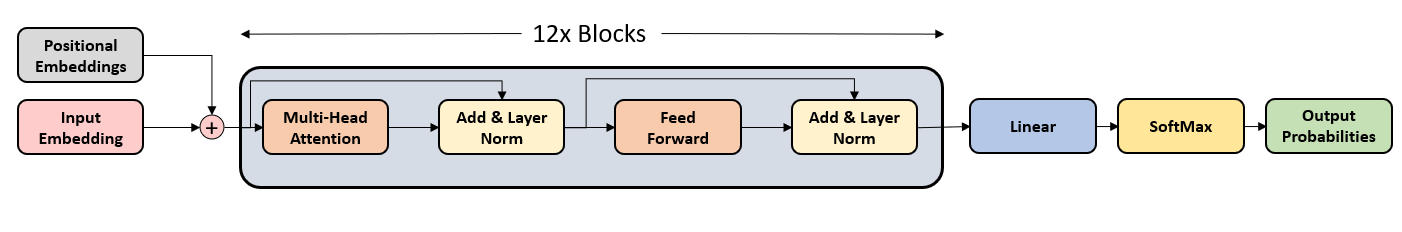
\includegraphics[width=0.99\linewidth]{GPT_1.png}
\captionof{figure}{\color{Teal} Generative Pre-trained Transformer Architecture.}
\end{center}\vspace{0.5cm}
\end{comment}

\color{Teal}

%%%%%%%%%%%%%% INTRODUCTION %%%%%%%%%%%%%%%%%%%%%%%%%%%%%
\section*{Introduction}
\color{Black}

Cognitive distortions are irrational or biased ways of thinking that can contribute to negative emotions and behaviors. 
Cognitive-behavioral therapy (CBT) is a common therapeutic approach that aims to help individuals identify and challenge these distortions.
Detecting cognitive distortions from patient-therapist interactions is a challenging task that has been addressed in recent research, and could be crucial in many types of 
therapy to help therapstis and individuals identify and challenge these distortions.
Prior research has attempted to use a dataset of human-labeled patient-therapist interactions to train a model to detect cognitive distortions\cite{original_paper}.
However, the dataset is highly imbalanced, with the majority of the data belonging to the non-distorted class, which poses a challenge for predictive modeling.
Generative AI models have the potential to address class imbalance by generating new data for the minority classes.
In this study, we explore the use of generative AI models to address class imbalance in cognitive distortion predictive models
by comparing the performance of different generative AI models, vectorizers, and classification algorithms on the task of detecting cognitive distortions from patient-therapist interactions.
We consider both binary and multi-class classification tasks and evaluate the models using the weighted F1-score as the performance metric.

%%%%%%%%%%%%%% INITIAL DATA ANALYSIS %%%%%%%%%%%%%%%%%%%%%%%%%%%%%
\color{Teal}
\section*{Initial Data Analysis}
\color{Black}

We use a dataset of patient-therapist interactions to train our models.
The dataset contains 10 classes of cognitive distortions, with the majority of the data belonging to the non-distorted class.
We first treat the problem as a binary classification task, where we combine all the distorted classes into a single class and compare the performance of 
different classification algorithms.
We use the Term Frequency-Inverse Document Frequency (tf-idf) vectorizer to convert the text data into numerical features and train a 
Linear Support Vector Classifier (LinearSVC) on the data.
The best initial F1-score for the binary classification task is 0.73 using tf-idf and LinearSVC.
We then treat the problem as a multi-class classification task and compare the performance of different classification algorithms.
The best initial F1-score for the multi-class classification task is 0.21 using tf-idf and LinearSVC.
The addition of the non-distorted class to the multi-class classification task resulted in a marginal improvement in performance, 
with an F1-score of 0.32 using tf-idf and LinearSVC.


\begin{center}\vspace{0.5cm}
	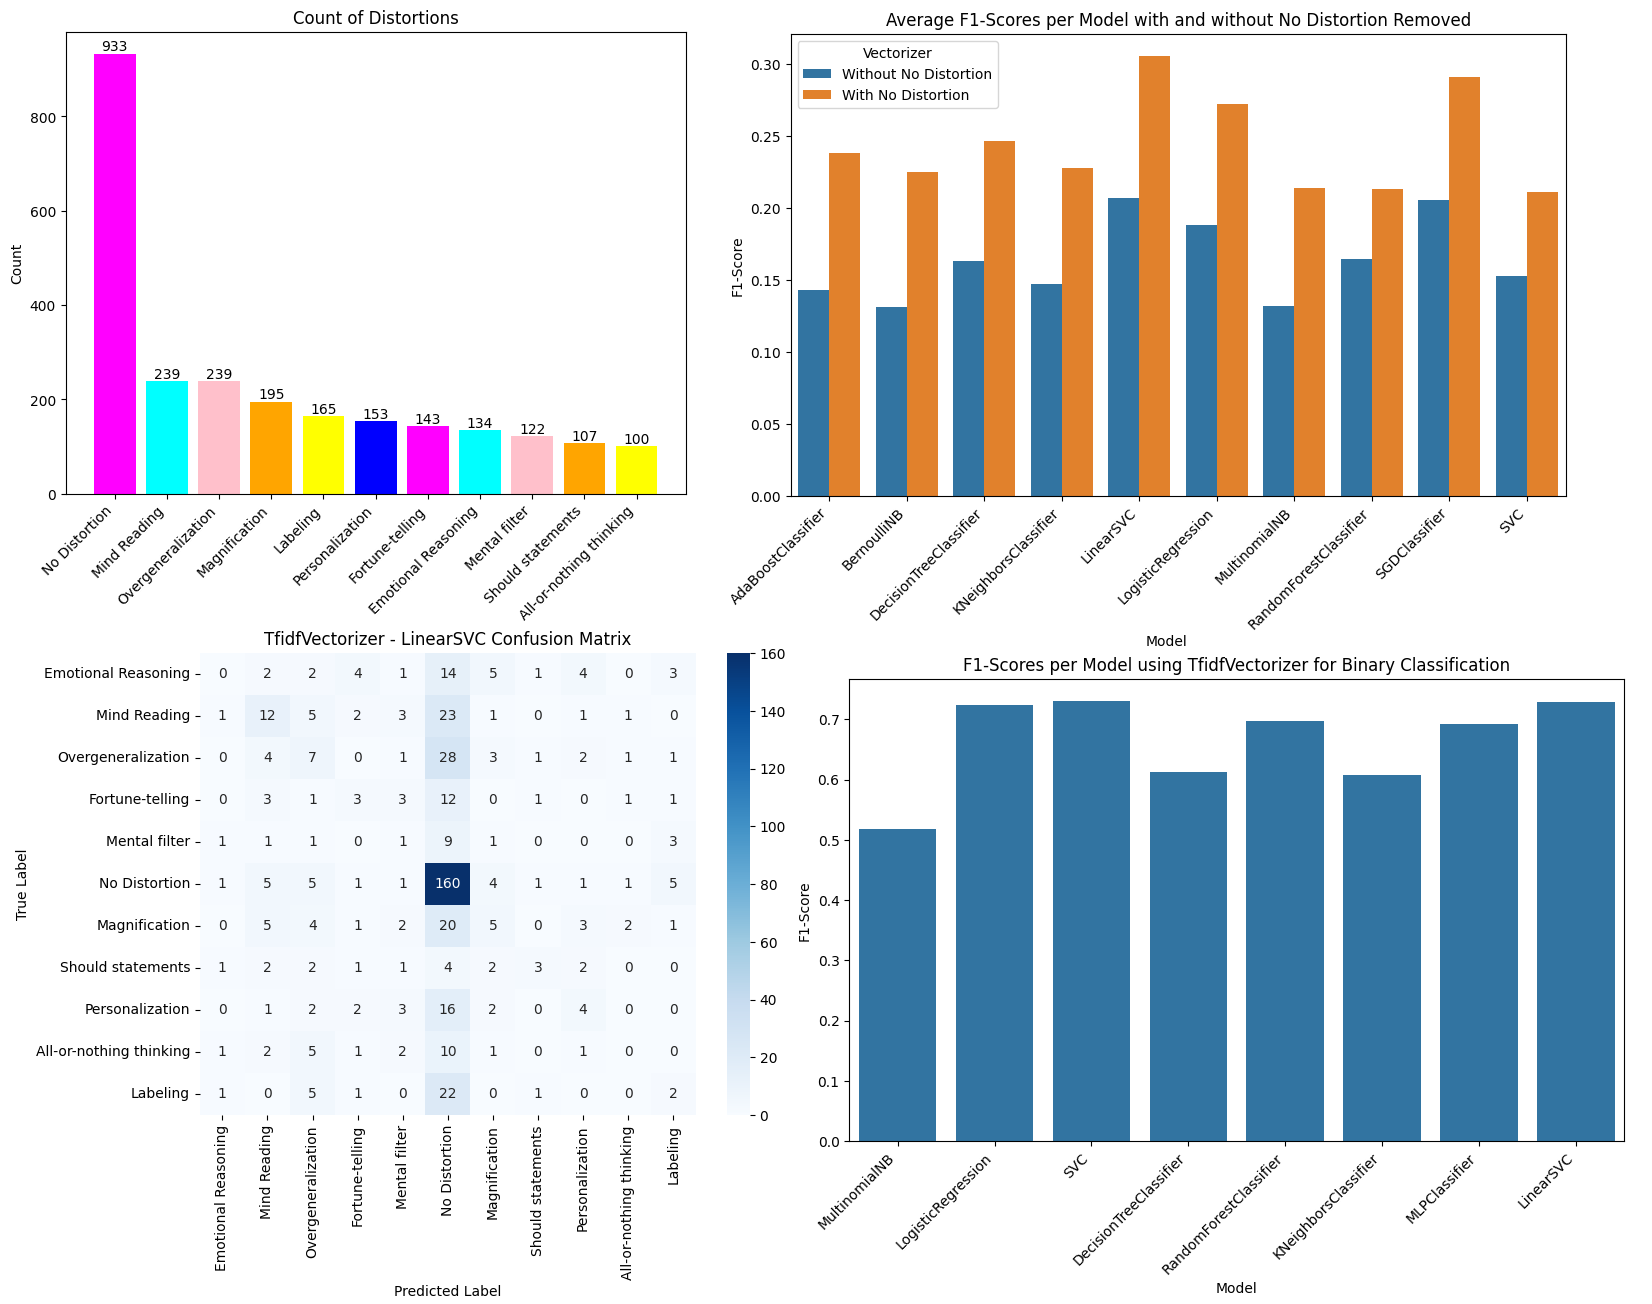
\includegraphics[width=0.99\linewidth]{figures/1stFour.png}
	\label{figure1}
	\captionof{figure}{\color{Teal} (Top-Left) Class Imbalance; (Top-Right) Average F1-Scores with and without No Distortion data; (Bottom-Left) Confusion Matrix of best model with No Distortion data; (Bottom-Right) F1 Scores for Binary Classification}
\end{center}\vspace{0.5cm}

%%%%%%%%%%%%%% SBERT EMBEDDINGS %%%%%%%%%%%%%%%%%%%%%%%%%%%%%
\color{Teal}
\section*{Sentence-BERT Embeddings}
\color{Black}

Sentence-BERT (SBERT) is a variant of the BERT model that is specifically trained to generate sentence embeddings. 
We compare the performance of different SBERT models on the task of detecting cognitive distortions from patient-therapist interactions. 
We use the Sentence Transformer library to generate SBERT embeddings for the text data and train different classification algorithms on the embeddings. 
The best F1-score for the multi-class classification task is 0.262 using the "intfloat/multilingual-e5-large-instruct" (Multilingual) SBERT model and LinearSVC. 
The best F1-score for the binary classification task is 0.756 using the same SBERT model with SVM.

\begin{center}\vspace{1cm}
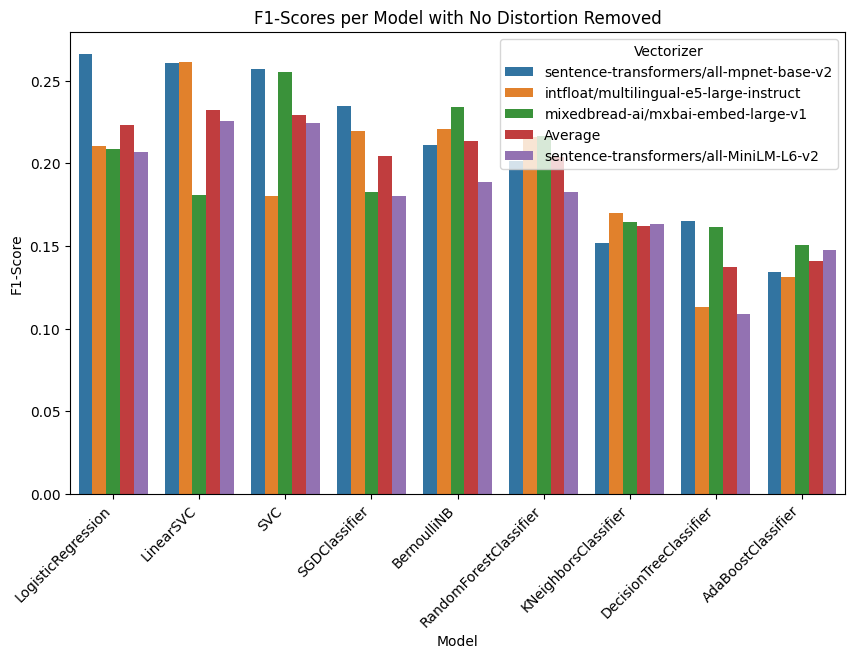
\includegraphics[width=0.81\linewidth]{figures/F1ScoresInitSBERT.png}
\captionof{figure}{\color{Teal} F1-Scores for SBERT Models}
\end{center}

\color{Black}

%%%%%%%%%%%%%% GENERATIVE AI MODELS %%%%%%%%%%%%%%%%%%%%%%%%%%%%%
\color{Teal}
\section*{Generative AI Models}
\color{Black}

We explore the use of generative AI models to address class imbalance in cognitive distortion predictive models. 
For the first set of experiments, we use the "mistralai/Mistral-7B-Instruct-v0.2" (Mistral) model to generate new records for the minority classes in the dataset.
We used a recursive technique to generate new records taking the generated data and appending the same question and feeding it back to the model, extracting and storing 
the generated data.
We then used a sampling technique by pulling three random samples from the generated data, acting as if the model generated that data, and asking the model to generate 
a fourth sample similar to the three and including the distortion with it.
We used this sampling technique on GPT-4 as it was the most inexpensive, the fastest, and the cleanest method to generate data, although later we found that it was not 
the most effective.
Results show that the addition of generated data using the Mistral model with recursive data generation on the binary classification task resulted in
the highest F1-score boost for both the binary and multi-class classification tasks, with the ladder results shown below.

\begin{center}
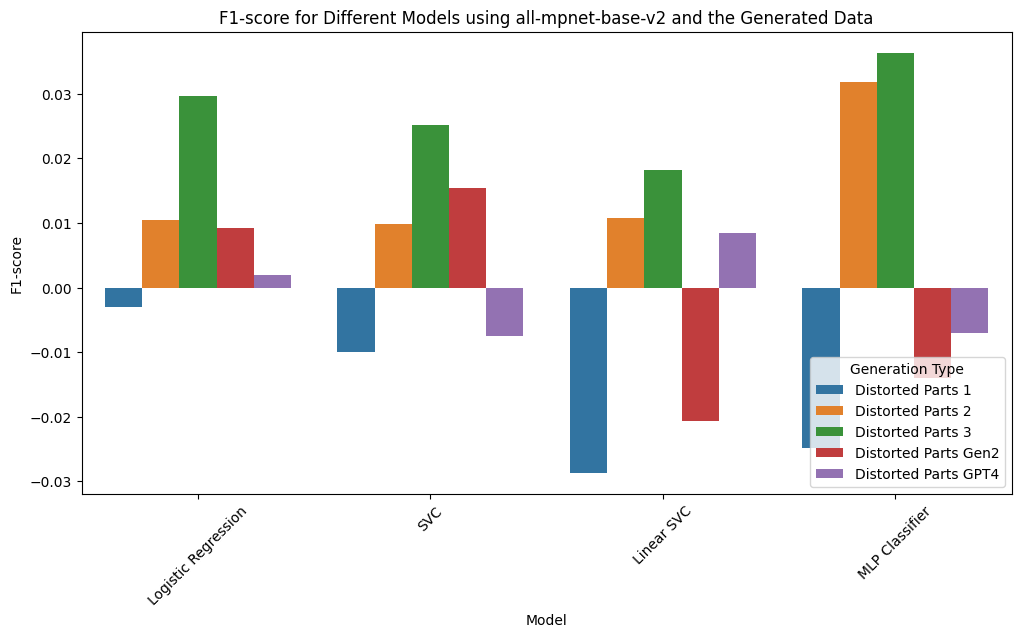
\includegraphics[width=0.96\linewidth]{figures/generatedDataDiffDiff.png}
\captionof{figure}{\color{Teal} Average Difference in F1-Score from baseline tests (no added generated data) for Different Generation Techniques and Classification Tasks}
\end{center}\vspace{1cm}


%%%%%%%%%%%%%% RESULTS AND EVALUATION %%%%%%%%%%%%%%%%%%%%%%%%%%%%%
\color{Teal}
\section*{Results and Evaluation}
\color{Black}

The best F1-score for the multi-class classification task is 0.298 using the Multilingual SBERT model and MLPClassifier with hyperparameter tuning and recursive generated Mistral data 2. 
The best F1-score for the binary classification task is 0.765 using the Multilingual SBERT model and SVM with hyperparameter tuning and recursive generated Mistral data 2. 

\begin{center}
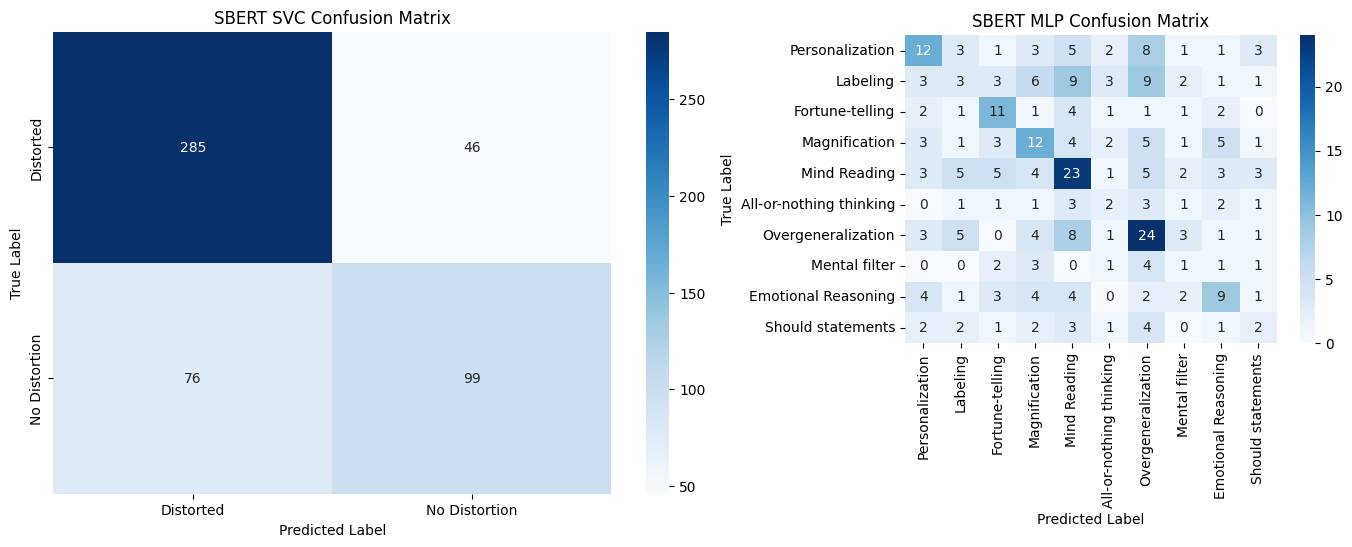
\includegraphics[width=0.96\linewidth]{figures/finalGraphs.png}
\captionof{figure}{\color{Teal} Confusion Matrix of best models' performance on the binary (left) and multi-class (right) classification task}
\end{center}\vspace{1cm}

%%%%%%%%%%%%%% DISCUSSION %%%%%%%%%%%%%%%%%%%%%%%%%%%%%
\color{Teal}
\section*{Discussion}
\color{Black}
The inter-annotator agreement (IAA) score posed a challenge in this study, as the human annotators had difficulty agreeing on the labels for the data (Table~\ref*{origCounts}). 
This may have affected the performance of the generative AI models. 
The best model we have found for detecting cognitive distortions from patient-therapist interactions is the Multilingual SBERT model with SVM classification and hyperparameter tuning, 
achieving an F1-score of 0.765. 
The best model we have found for classifying the data into the 10 classes is the Multilingual SBERT model with MLPClassifier and hyperparameter tuning, achieving an F1-score of 0.298.
\vspace{0.5cm}

Future work includes exploring different methods of text 
generation and categorization, such as fine-tuning other large language models and prompt engineering techniques to generate more data, potentially yielding higher F1-scores.

\begin{center}\vspace{0.1cm}
\centering
\begin{tabular}{|l|c|}
\toprule
\textbf{Cognitive Distortion} & \textbf{\begin{tabular}[c]{@{}l@{}}Percentage of Records \\ containing a Secondary Distortion\end{tabular}} \\
\midrule
All-or-Nothing Thinking       & 23\%                                                                                                        \\\hline
Emotional Reasoning           & 27\%                                                                                                        \\\hline
Fortune-Telling               & 29\%                                                                                                        \\\hline
Labeling                      & 38\%                                                                                                        \\\hline
Magnification                 & 26\%                                                                                                        \\\hline
Mental Filter                 & 34\%                                                                                                        \\\hline
Mind Reading                  & 17\%                                                                                                        \\\hline
Overgeneralization            & 22\%                                                                                                        \\\hline
Personalization               & 32\%                                                                                                        \\\hline
Should statements             & 20\%                                                                                                       \\\hline
\end{tabular}
\captionof{table}{\color{Teal} {Analysis of Secondary Distortions in Cognitive Distortions}
\label{origCounts}}
\end{center}

%%%%%%%%%%%%%% CONCLUSION %%%%%%%%%%%%%%%%%%%%%%%%%%%%%
\color{Teal}
\section*{Conclusion}
\color{Black}

In conclusion, the addition of generated data using the Mistral-7B-Instruct-v0.2 model with recursive data generation on the binary classification task 
resulted in a boost of 0.01 with an F1-score of 0.765 using the same SBERT embeddings with SVM classification model. 
On the other hand, the same additional data on the multi-class classification task resulted in a boost of 0.036 with an F1-score of 0.298 
using the same SBERT embeddings with MLPClassifier and hyperparameter tuning.
The binary classification task is useful for a future system and would be a good first step for further analysis by a human, but there is lots more work to be done 
within this field and this project.

%%%%%%%%%%%%%% ACKNOWLEDGEMENTS %%%%%%%%%%%%%%%%%%%%%%%%%%%%%
\color{Teal}
\section*{Acknowledgements}
\color{Black}

We would like to acknowledge the support of the QUEST Program and Dr. Lauren for their guidance and assistance throughout this research project.

%%%%%%%%%%%%%% REFERENCES %%%%%%%%%%%%%%%%%%%%%%%%%%%%%
\color{Teal}
\begin{thebibliography}{9}
\color{Black}

\bibitem{original_paper}
Detecting Cognitive Distortions from Patient-Therapist Interactions. (2021). \textit{ACL Anthology}. Retrieved from https://aclanthology.org/2021.clpsych-1.17.pdf
\end{thebibliography}

\end{multicols}
\end{document}